\documentclass[11pt]{article}
\usepackage{graphicx}
\usepackage{geometry}
\usepackage{float}
\usepackage{amsmath}
\usepackage{circuitikz}
\usepackage{amssymb}
\usepackage{mathtools}
\usepackage{tikz}
\usepackage{cite}
\DeclarePairedDelimiter{\set}{\{}{\}}

\title{Charge to Mass Ratio of the Electron}
\author{Spandan Suthar}
\date{October 13, 2025}

\geometry{margin=1in}
\setlength{\parindent}{0pt}

\begin{document}

\maketitle

\section{Introduction and Background}

% TODO: is this introduction too basic?
In 1897, J.J. Thompson performed an experiment
that produced
beams of electrons from a thermally excited metal and deflected them using a
magnetic field, causing them to follow circular paths.
In doing so, he justified that these emissions are composed of
constituents with both charge and mass: experiencing an interaction
from a magnetic field while moving supported that these beams' constituents had
nonzero charge, and traveling in a circular arc with nonzero radius
caused by a force from a magnetic field supported that that they had
nonzero mass.
Thompson continued, obtaining a value of the charge to mass ratio
of the beam constituents that was consistent across different heated metals.
This result validated the notion of an electron as a fundamental
particle that is the same across the materials it is found in
\cite{thomp, young}.  In this experiment deriving from Thompson's
original procedure, the ratio of the
electron's charge to mass $\frac{e}{m}$ is determined by measuring the radius of
the circular path of the electrons in a magnetic field produced by a pair of
Helmholtz coils.

% TODO: it's necessary to briefly describe system here; equations hinge on it.
% Or should we aim for abstract description?

\vspace{1em}

As part of this experiment, electrons initially at potential $V_0 = 0$ are
accelerated by an anode with potential $V_a$ and freely pass
through a space with a uniform magnetic field $\vec B$. The Lorentz
force on an electron with charge $-e$ moving with velocity $\vec v$
through this magnetic field $\vec B$ and negligible electric field is
given by \cite{griff, young}:

\begin{equation}
  \label{eq:lorentz_force}
  \vec{F} = -e \vec{v} \times \vec{B}
\end{equation}

% TODO: any previous derivations necessary? Need to include the
% energy equations?
Because this force is orthogonal to the electron's velocity
and to the field direction, the electrons travel in a circular arc
in the plane normal to the field direction. Using conservation of
energy principles and the uniform circular motion radial acceleration
constraint, the radius of this arc $r$, the anode
voltage $V_a$, the
magnetic field strength $B$ within the coils, the elementary charge $e$, and the
electron mass $m$ are related by \cite{thomp, young}:

\begin{equation}
  \label{eq:lin_regress}
  2V_a = \left ( \frac{e}{m} \right ) B^2 r^2
\end{equation}

\vspace{1em}

A pair of Helmholtz coils is used to generate the uniform magnetic
field the electrons experience. The magnetic field strength $B$
within the coils causing the
circular acceleration can be
expressed as a function of the current $I$ through the coils, the number of
turns $N$, the diameter $D$, and the vacuum
permeability $\mu_0$ \cite{helm}:

\begin{equation}
  \label{eq:magnetic_field_equation}
  B = \frac{16 \mu_0 N I }{\sqrt{125} D}
\end{equation}

\section{Methodology}

An experimental setup is shown in Figure \ref{fig:apparatus}. A pair
of Helmholtz coils encloses a coordinate grid positioned next to an
anode, in which a slit is cut and through which electrons freed from a
filament can pass \cite{thomp, young}. The coils are supplied a
current via a DC power supply,
at which point a current through the coils can be measured
\cite{helm, young}. The anode is raised
to a voltage $V_a$ on the order of kilovolts, while the filament is
held at a potential on the order of volts. This causes freed electrons to
flow into the space in front of the coordinate grid and form a circular arc
according to Equation \ref{eq:lorentz_force}. A pair of
electrodes above and below the coordinate grid, raised to the same
large potential as the anode, ensure the electric field influence on
the electron
path is negligible \cite{griff}. The space within the coils is evacuated to a
vacuum to minimize electron scattering by air molecules and to ensure the only
acceleration on the electrons is only due to the magnetic field.

\begin{figure}[H]
  \centering
  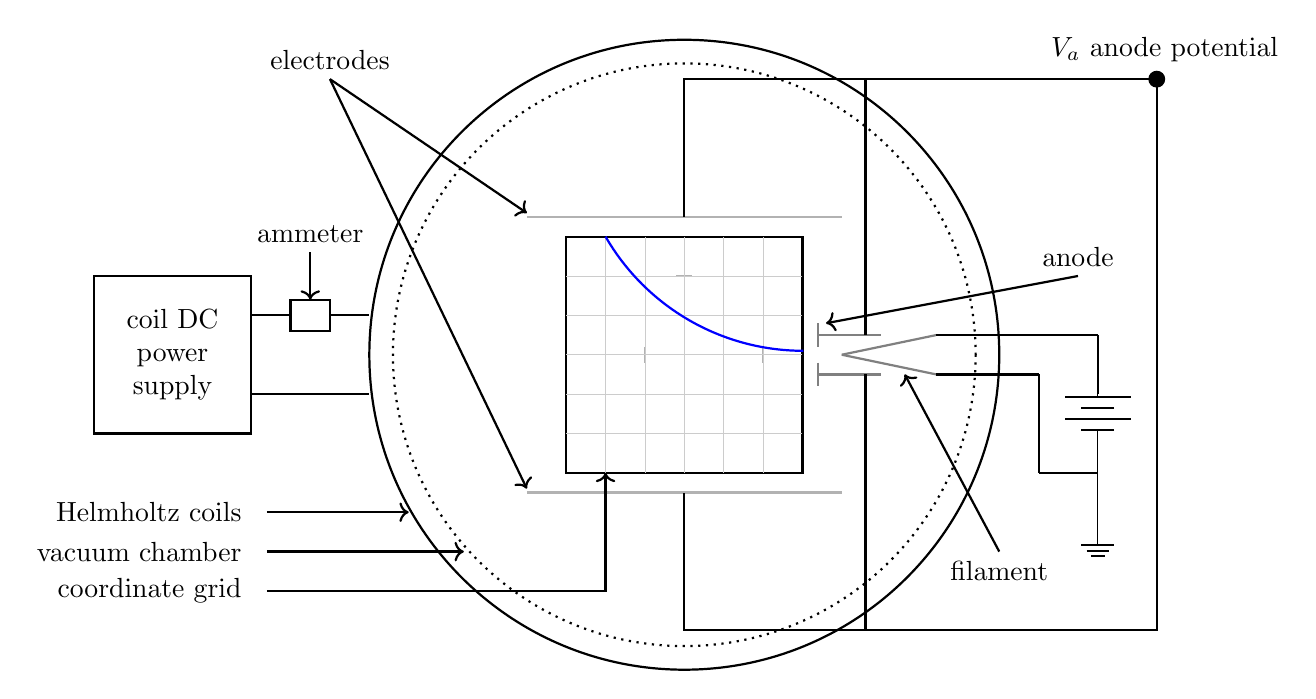
\begin{tikzpicture}
    % Draw the coil DC power supply box on the left side
    \draw[thick] (-7.5,-1.0) rectangle (-5.5,1.0);
    \node[text width=1.5cm, align=center] at (-6.5,0) {coil DC power supply};

    % Draw leads from the power supply box to the Helmholtz coils
    \draw[thick] (-5.5,0.5) -- (-5.0,0.5);
    \draw[thick] (-5.0,0.3) rectangle (-4.5,0.7);

    % Add ammeter label with arrow above the small box on the lead
    \node[above] at (-4.75,1.3) {ammeter};
    \draw[thick, ->] (-4.75,1.3) -- (-4.75,0.7);

    \draw[thick] (-4.5,0.5) -- (-4.0,0.5);
    \draw[thick] (-5.5,-0.5) -- (-4.0,-0.5);
    % Draw the circle for Helmholtz coils
    \draw[thick] (0,0) circle (4cm);
    % Add inner dotted circle
    \draw[thick, dotted] (0,0) circle (3.7cm);
    % Draw border around coordinate grid
    \draw[thick, black] (-1.5,-1.5) rectangle (1.5,1.5);
    % Draw horizontal lines above and below the grid that are slightly wider
    \draw[thick, gray!60] (-2.0,1.75) -- (2.0,1.75);
    \draw[thick, gray!60] (-2.0,-1.75) -- (2.0,-1.75);
    % Add electrodes label with two arrows
    \node[above] at (-4.5,3.5) {electrodes};
    \draw[thick, ->] (-4.5,3.5) -- (-2.0,1.80);
    \draw[thick, ->] (-4.5,3.5) -- (-2.0,-1.70);
    % Draw coordinate grid without numbers
    \draw[thin, gray!60] (-1.5,0) -- (1.5,0);
    \draw[thin, gray!60] (0,-1.5) -- (0,1.5);
    % Add tick marks on axes (without numbers)
    \foreach \x in {-1,-0.5,...,1} {
      \draw[gray!60] (\x,0.1) -- (\x,-0.1);
    }
    \foreach \y in {-1,-0.5,...,1} {
      \draw[gray!60] (0.1,\y) -- (-0.1,\y);
    }
    % Add grid lines
    \foreach \x in {-1,-0.5,...,1} {
      \draw[very thin, gray!40] (\x,-1.5) -- (\x,1.5);
    }
    \foreach \y in {-1,-0.5,...,1} {
      \draw[very thin, gray!40] (-1.5,\y) -- (1.5,\y);
    }
    % Plot part of an arc centered off the grid, starting horizontally
    % and bending upward
    \draw[thick, blue, -] (-1.0,1.50) arc (210:270:2.9);
    % Add the T-shaped objects on the right side of the grid
    % First T-shape (upper)
    \draw[thick, gray] (1.7,0.25) -- (2.5,0.25);
    \draw[thick, gray] (1.7,0.1) -- (1.7,0.4);
    % Second T-shape (lower)
    \draw[thick, gray] (1.7,-0.25) -- (2.5,-0.25);
    \draw[thick, gray] (1.7,-0.1) -- (1.7,-0.4);
    % Add the wedge-shaped object (filament) between the T-shapes
    \draw[thick, gray] (2.0,0) -- (3.2,0.25);
    \draw[thick, gray] (2.0,0) -- (3.2,-0.25);
    % Add circuit leads from the filament
    \draw[thick] (3.2,0.25) -- (5.25,0.25);   % Top lead horizontal
    \draw[thick] (5.25,0.25) -- (5.25,-0.5);   % Top lead down to battery
    \draw (5.25,-0.5) to[battery] (5.25,-1.0); % Battery
    \draw (5.25,-1.0) -- (5.25,-2.0); % Battery down to ground

    \draw[thick] (3.2,-0.25) -- (4.5,-0.25); % Bottom lead horizontal
    \draw[thick] (4.5,-0.25) -- (4.5,-1.5);  % Bottom lead down
    \draw[thick] (4.5,-1.5) -- (5.25,-1.5);   % Bottom lead rightward
    \node[ground] at (5.25,-2.0) {}; % Add ground symbol

    % Add dot for Voltage (V_a) and connect it to the grid's top horizontal line
    \draw[fill=black] (6.0,3.5) circle (0.1cm);
    \draw[thick] (6.0,3.5) -- (0.0,3.5) -- (0.0,1.75);

    % New elbow connector entering bottom plate
    \draw[thick] (6.0, 3.5) -- (6.0,-3.5) -- (0.0,-3.5) -- (0.0,-1.75);

    % New horizontal branch from V_a dot to top T object
    \draw[thick] (6.0,3.5) -- (2.3,3.5) -- (2.3,0.25);

    % New horizontal branch from V_a dot to bottom T object
    \draw[thick] (6.0,-3.5) -- (2.3,-3.5) -- (2.3,-0.25);

    % Add anode label with arrow pointing to the top T-shape object
    \node[above] at (5.0, 1.0) {anode};
    \draw[thick, ->] (5.0, 1.0) -- (1.8, 0.40);

    % Add filament label with arrow pointing to the V-shaped object
    \node[below] at (4.0, -2.5) {filament};
    \draw[thick, ->] (4.0, -2.5) -- (2.8, -0.25);

    \node[above] at (6.1,3.6) {$V_a$ anode potential};

    \node[left] at (-5.5, -2.0) {Helmholtz coils};
    \draw[thick, ->] (-5.3, -2.0) -- (-3.5, -2.0); % Arrow to outer circle

    \node[left] at (-5.5, -2.5) {vacuum chamber};
    \draw[thick, ->] (-5.3, -2.5) -- (-2.80, -2.5); % Arrow to inner
    % dotted circle

    \node[left] at (-5.5, -3.0) {coordinate grid};
    \draw[thick, ->] (-5.3, -3.0) -- (-1.0, -3.0) -- (-1.0, -1.5); %
    % Arrow to coordinate grid

  \end{tikzpicture}
  \caption{The experimental setup used to deflect emitted electrons.
    A pair of Helmholtz coils produce a uniform magnetic field
    \cite{helm} through
    a coordinate grid, over which electrons freed from a
    thermally-excited filament can pass---indicating their path. The
    electrons are given an initial velocity by accelerating toward an anode,
    which is raised to a voltage $V_a$ \cite{young, griff}.
    Electrodes at potential $V_a$
    above and below the coordinate grid prevent electric field influences on the
    electron path by rendering potential gradients in the region
    negligible \cite{griff}. The space in which electrons travel is
    enclosed in a
    vacuum chamber. Current is supplied to the coils via a DC power
    supply, another voltage source heats the
    filament, and a high-voltage source provides the anode and
  electrode voltages.}
  \label{fig:apparatus}
\end{figure}

Anode voltages of $V_a = \space $\space  $1000$, $1500$, $2000$,
$2500$, and $3000$
volts are produced
and correspond to electron streams of various speeds--and thus to
Lorentz forces of different magnitudes. Once a stream
of electrons is established, the magnetic field of the coils is adjusted to
produce an arc of approximately the same $3.3$ cm radius as the arcs
in the sibling trials. This is done by targeting a particular
reference point on the path per trial. The coil current $I$
accomplishing this is recorded and $y$-coordinates on the arc
corresponding to the $x$-coordinates $[x_i]_i = [2.0,
4.0, 6.0, 8.0, 10.0]$ cm are measured using the coordinate grid.

\vspace{1em}

% TODO: to what detail should we discuss correcting for the V_offset?
% This is a little too specific to our setup.

% TODO: this seems specific to our approach. Should we describe
% averaging at all?
% TODO: should we include discussions about mirroring the situation and

It is possible that the anode slit does not align perfectly with the
$x$-axis of the coordinate grid or that other magnetic fields influence
the electron path. Two measures address these issues: correction using
zero-field offsets and reversal of the magnetic field.
The first measure involves the following: $y$-coordinates of the
electron path
without an active magnetic field are measured and
subtracted from the $y$-coordinate readings of the electron path with an
active magnetic field. The second measure is as follows: Upon
collecting arc $y$-coordinates across all voltages, the magnetic field is
reversed such that the electron path's $y$-coordinate is inverted. For each
anode voltage, the current is brought to the same magnitude as
in the corresponding non-inverted trial and coordinates of points on the
arc are again measured, corresponding to the same $x$-coordinates.
For each voltage, the entire data-collection process yields two lists
of $y$-coordinates: an original list $[\hat y_i]_i$ and the
inverted-field list $[\hat y_i']_i$.

\section{Results}

The $y$-coordinate magnitudes obtained from each trial and its
inverted-field counterpart are averaged, producing a single list of
$y$-coordinates:
$\left [ \frac{|\hat y_i| + |\hat y_i'|}{2} \right ]_i = \left [ y_i
\right ]_i$. Fitting a
circle's equation to the points $\left [ (x_i, y_i) \right ]_i$
yields one path radius
$r$ per anode voltage. Associated path radii, anode voltages,
and coil currents are shown in Table \ref{tab:results} and an example
of a circle fit to the coordinates of an electron path is displayed in Figure
\ref{fig:circle_fit}.

\vspace{1em}

For each anode voltage in Table \ref{tab:results},
a value of the electron charge to mass ratio $\frac{e}{m}$ is calculated using a
rearranged form of Equation \ref{eq:lin_regress}, with values of $B$
obtained from Equation \ref{eq:magnetic_field_equation} using a coil
turn number of 320 and a coil diameter of $(15.5 \pm
0.5)$ cm. These values are also shown in Table \ref{tab:results}.
Taking the mean of these
pointwise values and performing a standard deviation of mean analysis produces
an experimental value of $\frac{e}{m} = (1.68 \pm 0.05) \times 10^{11}$ C/kg.
The accepted CODATA value for $\frac{e}{m}$ lies within $2 \sigma$ of
this experimental value \cite{codata}.

\vspace{1em}

$\frac{e}{m}$ data points, the experimental value, and the accepted
CODATA value are displayed in Figure
\ref{fig:e_to_m_vs_anode_voltage}. Inspection of this plot reveals
that the trials
corresponding to anode voltages 2500 and 3000 volts produced values considerably
lower than the accepted value.

% TODO: Is it necessary to include the actual circle equation or center coords?

% TODO: radius uncertainty should be propagated through least squares,
% not through a single calculation.
\begin{table}[h!]
  \centering
  \begin{tabular}{c c c c c}
    Anode Voltage (V) ($\pm 1$ V) & $r$ (m) & $I$ (A) ($\pm 0.0001A$)
    & $e/m$ ($10^{11}$ C/kg) \\
    \hline
    1000 & $0.33 \pm 0.04$ & 0.0850 & $1.8 \pm 0.5$ \\
    1500 & $0.327 \pm 0.011$ & 0.1052 & $1.72 \pm 0.16$ \\
    2000 & $0.318 \pm 0.018$ & 0.1238 & $1.75 \pm 0.23$ \\
    2500 & $0.34 \pm 0.04$ & 0.1393 & $1.5 \pm 0.3$ \\
    3000 & $0.326 \pm 0.026$ & 0.1540 & $1.62 \pm 0.28$ \\
  \end{tabular}
  \caption{Measured values of anode voltage $V_a$, electron path
    radius $r$, coil current $I$, and calculated electron
  charge-to-mass ratio ($e/m$) for each trial.}
  \label{tab:results}
\end{table}
% TODO: better caption here
% TODO: does the circle fit diagram contain enough information?
\begin{figure}[H]
  \centering
  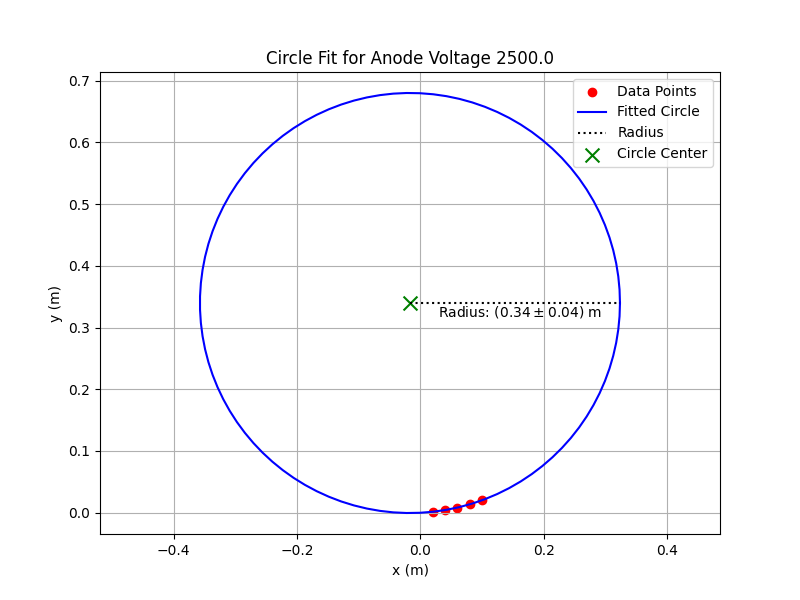
\includegraphics[width=1.0\textwidth]{../circle_fit_3.png}
  \caption{An example of a circle fit to points measured from an
    electron beam's path using least squares methods, with a radius
  obtained as a result of fitting.}
  \label{fig:circle_fit}
\end{figure}

% TODO: discuss sources of uncertainty
% TODO: account for offsets and propagate these uncertainties
% in the y-coordinate measurements

% TODO: caption
\begin{figure}[H]
  \centering
  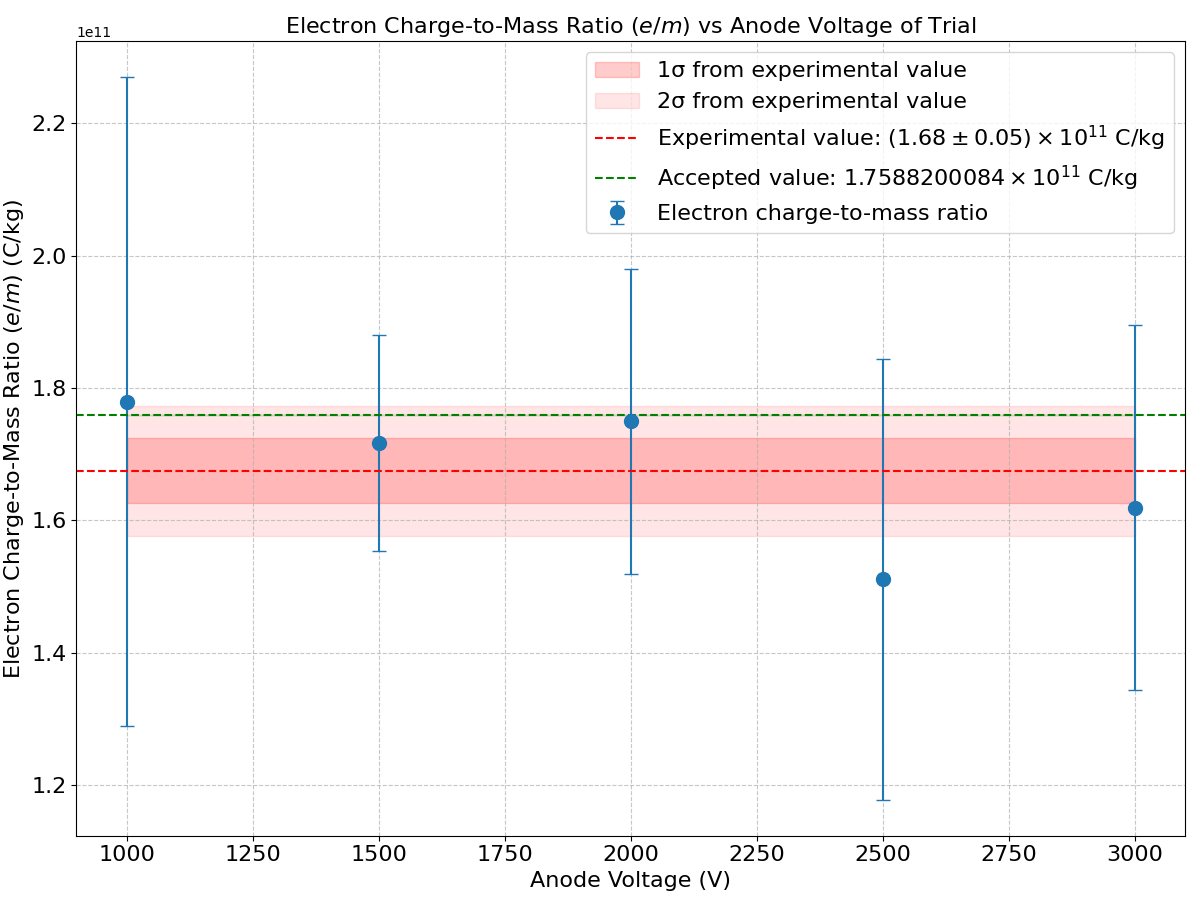
\includegraphics[width=1.0\textwidth]{../e_to_m_vs_anode_voltage.png}
  \caption{A plot indicating measured values of the electron charge
    to mass ratio derived
    from the values of $\frac{e}{m}$ in Table \ref{tab:results}. 1$\sigma$
    and 2$\sigma$ intervals around the dashed red experimental value
    are shaded in red, and the accepted CODATA value \cite{codata} is
    shown in green.
    Note that the points corresponding to anode voltages 2500 and 3000 volts
    are considerably lower than the accepted value.
  }
  \label{fig:e_to_m_vs_anode_voltage}
\end{figure}

% TODO: include plot for linear regression fit

\section{Conclusion and Discussion}

This experiment finds a value of the electron charge to mass ratio,
$(1.68 \pm 0.05) \times 10^{11}$ C/kg, that is in agreement
with the accepted CODATA value to within $2 \sigma$. It is possible that the
electrodes above and below the coordinate grid were not perfectly
aligned or that there are imperfections in the electrode materials, resulting
in asymmetric electric field effects between the original trials and the
field-flipped trials. Uniform magnetic fields are also a physical
ideal; the coils' field might have had non-uniformities from one point on the
coordinate grid to another \cite{helm, young}. Any of these
factors could have created a path that
is not entirely circular, invalidating equation \ref{eq:lin_regress},
which assumes uniform circular motion.

\vspace{1em}

In particlar, it was noticed that paths with inverted fields tended to have
larger $y$-coordinates than paths with non-inverted fields. A
negligible zero-field deflection was observed, suggesting that this
asymmetry could be due to the aforementioned non-uniformities in the magnetic
field or in the electrodes' effects.

\vspace{1em}

Qualitatively, it is noted that the electron beams follow roughly circular arcs
through the magnetic field in agreement with the theoretical
acceleration they would experience from the Lorentz force described by
Equation \ref{eq:lorentz_force}: for a leftward-pointing initial electron
velocity $\vec v_0$ and a magnetic field $\vec B$ pointing into the coordinate
grid, the electrons experience a force antiparallel with the cross product
$\vec v_0 \times \vec B$---or downward along the coordinate grid.

\bibliographystyle{plain}
\bibliography{references}

\end{document}
